%!TEX root = ../main.tex

% Appendix Template

\chapter{Experiments on HDD drives} % Main appendix title
\label{Appendix-B} % Change X to a consecutive letter; for referencing this appendix elsewhere, use \ref{AppendixX}

The following experiments were conducted in an HDD drive which was benchmarked to have a random-write bandwidth of 1.2 MB/s and a sequential-write bandwidth of 2.7 MB/s with the \verb|fio| tool.

The intention behind conducting this experiment was to evaluate whether slower rotational magnetic hard drives can influence the results in Chapter \ref{Chapter4-evaluation}. The experiments in Chapter \ref{Chapter4-evaluation} were conducted in an NVMe SSD drive which is faster and non-rotational.

It seems that these characteristics do not have an impact on the outcome. The diagrams are visually similar (because the random seeds are the same), they are just ``shifted slightly upwards'' because the drive is slower.

The absence of any significant difference in the results can be justified by the fact that all stores write data sequentially, not randomly, and sequential writes are similar to both types of drives in the sense that they are both fast. It's random writes that degrade the performance of rotational HDDs because the disk head must move and wait for the disk to rotate, and this type of writes are not used in our use-case.

\section{Compaction in AppendLog}

\begin{figure}[h]
    \centering
    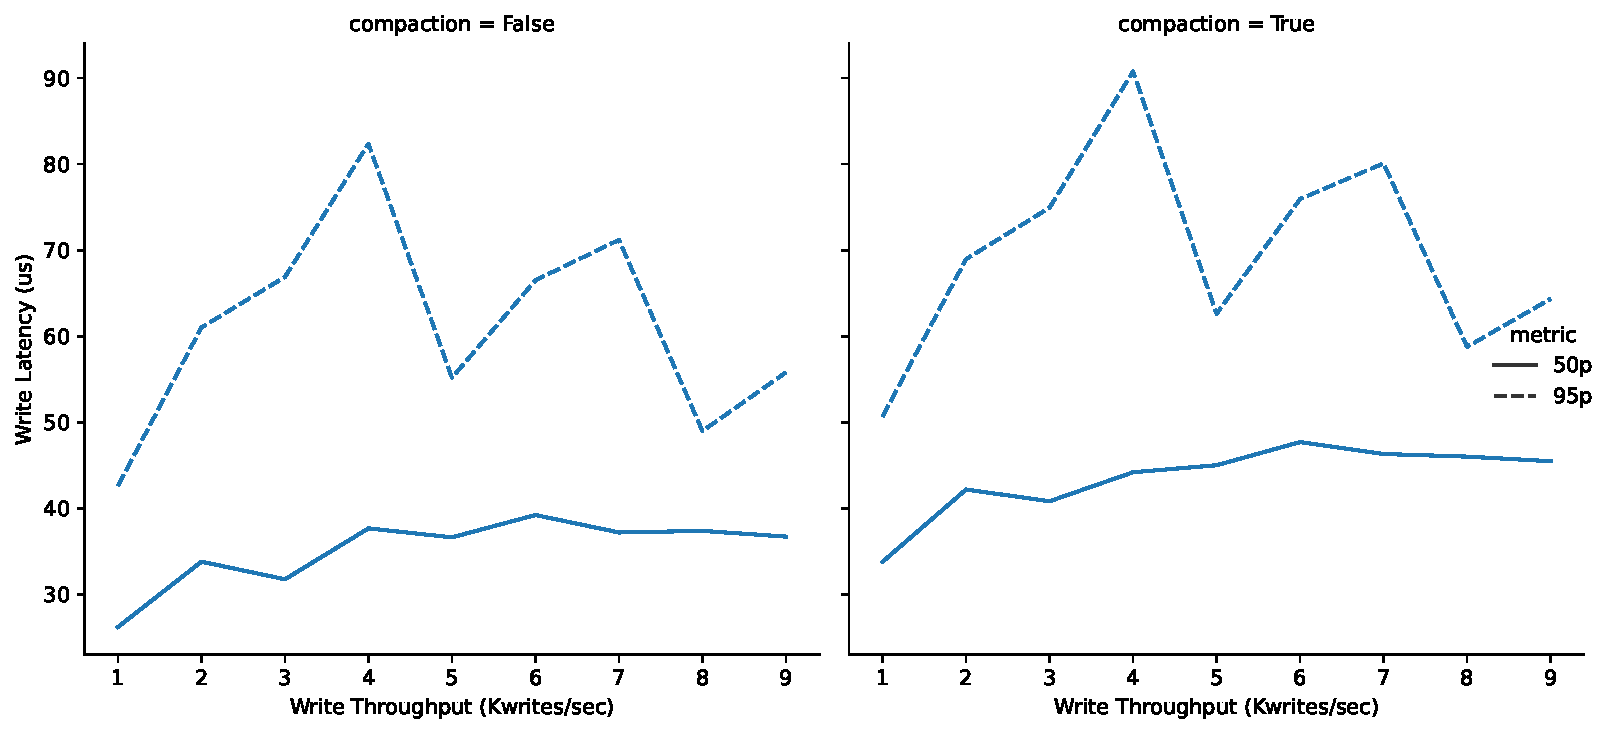
\includegraphics[width=1\textwidth]{compaction_write-hdd.pdf}
    \caption{Writes in AppendLog with compaction disabled (left) and enabled (right) in an HDD.}
    \label{fig:compaction-write-hdd}
\end{figure}

\begin{figure}[h]
    \centering
    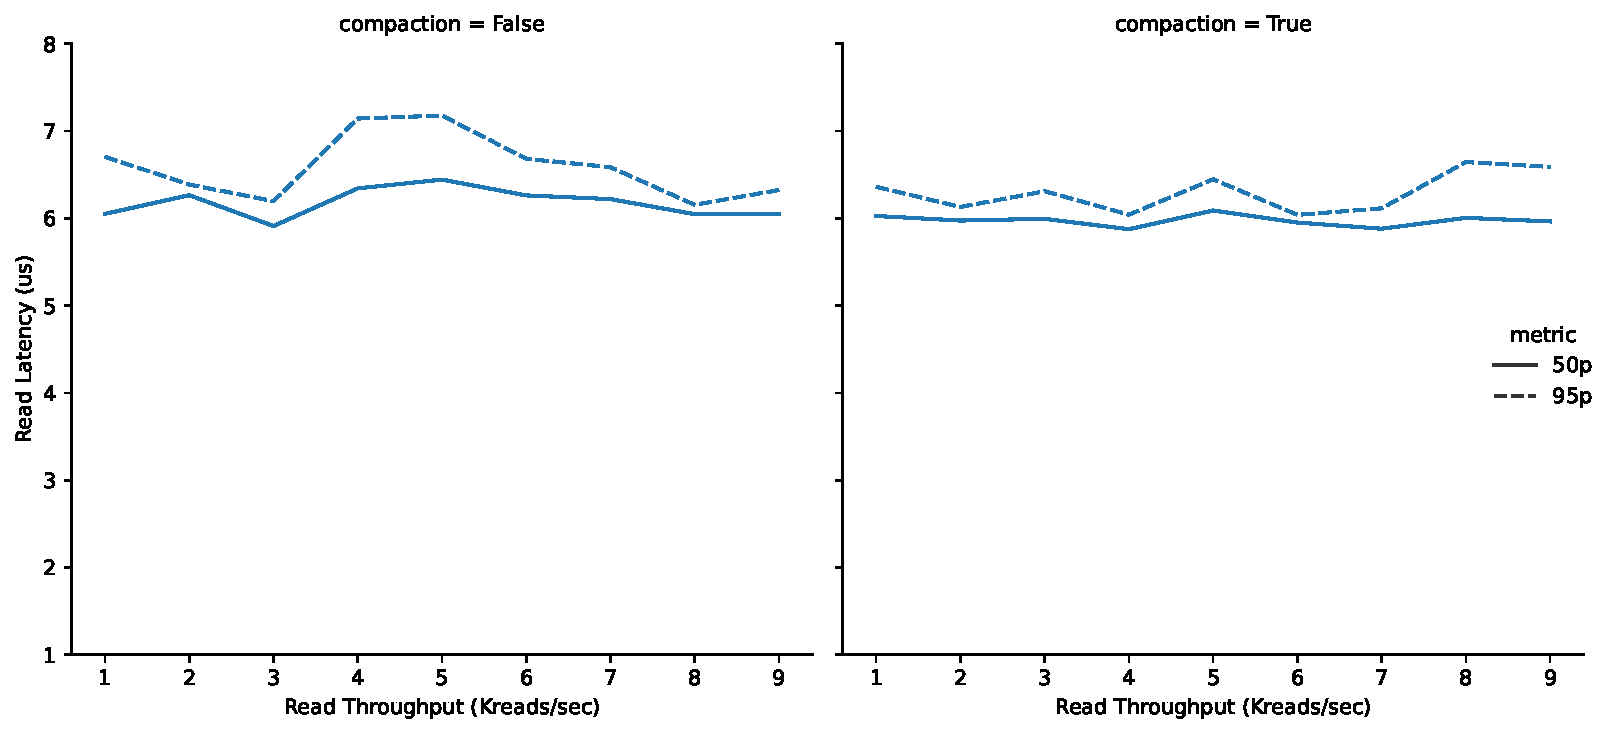
\includegraphics[width=1\textwidth]{compaction_read-hdd.pdf}
    \caption{Reads in AppendLog with compaction disabled (left) and enabled (right) in an HDD.}
    \label{fig:compaction-read-hdd}
\end{figure}

\section{Latencies}

\begin{figure}[h]
    \centering
    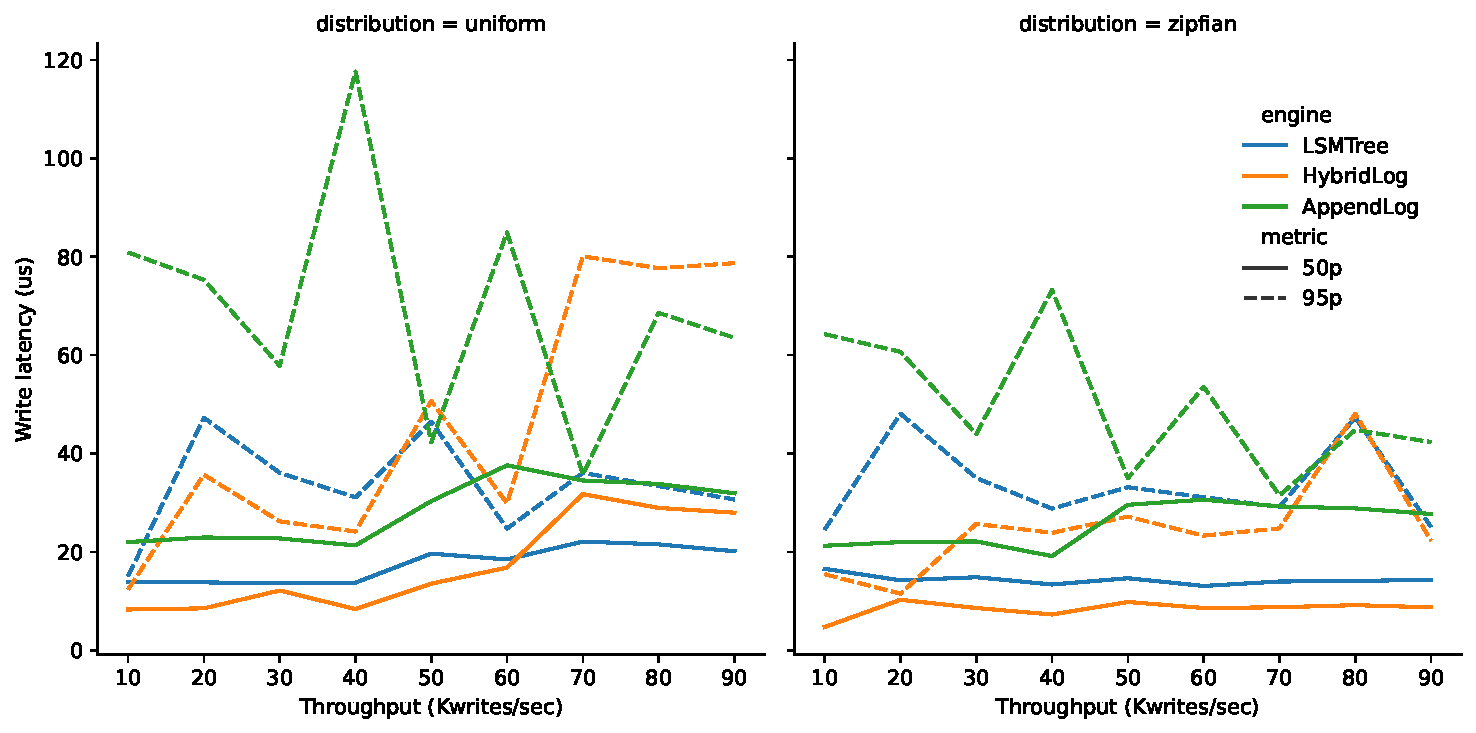
\includegraphics[width=1\textwidth]{write-throughput-hdd.pdf}
    \caption{Write latency for every store in an HDD.}
    \label{fig:write-throughput-hdd}
\end{figure}

\begin{figure}[h]
    \centering
    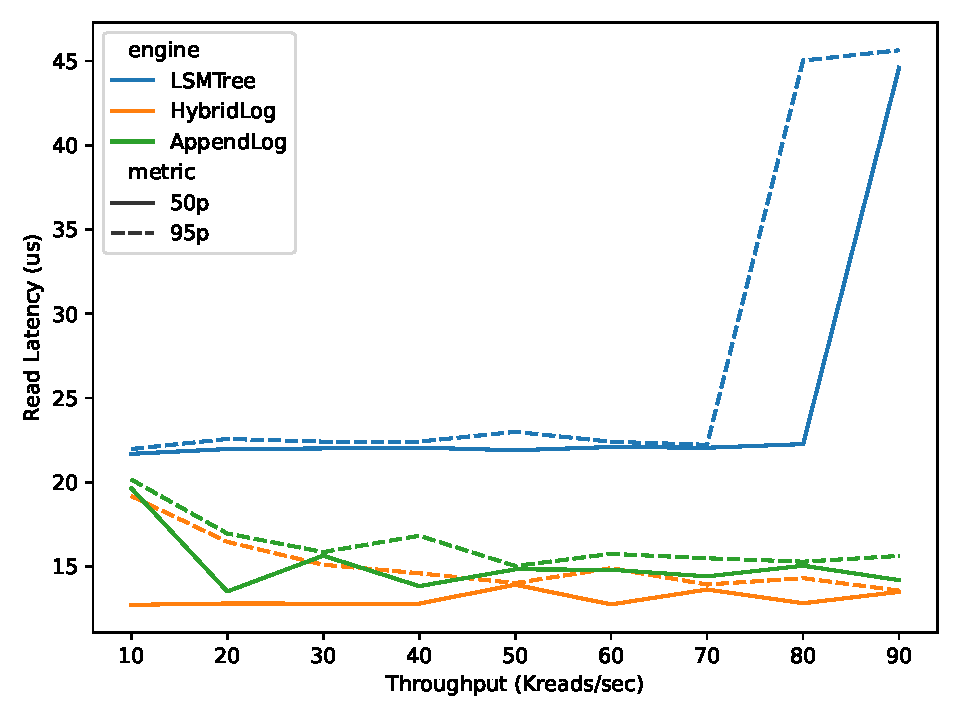
\includegraphics[width=0.6\textwidth]{read-throughput-hdd.pdf}
    \caption{Read latency for every store in an HDD.}
    \label{fig:}
\end{figure}
